\documentclass{beamer}

\usetheme{Baba}

\usepackage{emoji}

\usetikzlibrary{overlay-beamer-styles}

\hypersetup{
  colorlinks=true,
  urlcolor=blue,
  linkcolor=babadarkblue,
  citecolor=blue
}
\renewcommand{\UrlFont}{\normalfont}


\title{Supporting the treatment of Alzheimer's patients with explainable artificial intelligence}
\date{\today}
\author{Esten H. Leonardsen}

\begin{document}
    \begin{frame}
        \titlepage
    \end{frame}

    \newcommand{\mriside}[4]{
    \def\mridepth{0.75}

    \node[inner sep=0pt] (input) at (#1, #2) {
        \includegraphics[height=#3, width=#3]{#4}
    };

    \draw[fill=black] (input.north west) --
        ($ (input.north west) + (0.5 * \mridepth, 0.5 * \mridepth) $) --
        ($ (input.north east) + (0.5 * \mridepth, 0.5 * \mridepth) $) --
        (input.north east) -- cycle;
    \draw[fill=black] (input.north east) --
        ($ (input.north east) + (0.5 * \mridepth, 0.5 * \mridepth) $) --
        ($ (input.south east) + (0.5 * \mridepth, 0.5 * \mridepth) $) --
        (input.south east) -- cycle;
    \draw[] (input.north west) --
        ($ (input.north west) - (0.5 * \mridepth, 0.5 * \mridepth) $) --
        ($ (input.south west) - (0.5 * \mridepth, 0.5 * \mridepth) $) --
        (input.south west) -- cycle;
    \draw[] (input.north east) --
        ($ (input.north east) - (0.5 * \mridepth, 0.5 * \mridepth) $) --
        ($ (input.south east) - (0.5 * \mridepth, 0.5 * \mridepth) $) --
        (input.south east) -- cycle;
    \draw[] ($ (input.north west) - (0.5 * \mridepth, 0.5 * \mridepth) $) --
        ($ (input.north east) - (0.5 * \mridepth, 0.5 * \mridepth) $);
    \draw[] ($ (input.south west) - (0.5 * \mridepth, 0.5 * \mridepth) $) --
        ($ (input.south east) - (0.5 * \mridepth, 0.5 * \mridepth) $);
}


\newcommand{\inputside}[3]{
    \mriside{#1}{#2}{#3}{data/mri_sagittal.png}
}

\newcommand{\heatmapside}[3]{
    \mriside{#1}{#2}{#3}{data/combined_sagittal.png}
}

\newcommand{\convside}[6]{
    \def\sidex{#1}
    \def\sidey{#2}
    \def\sidewidth{#3}
    \def\sideheight{#4}
    \def\sidefillcolour{#5}
    \def\sidename{#6}

    \node[
        fill=\sidefillcolour,
        inner sep=0pt,
        outer sep=0pt,
        minimum width=\sidewidth,
        minimum height=\sideheight,
        draw=black
    ] (\sidename) at (\sidex, \sidey) {};
}

\newcommand{\convtop}[4]{
    \def\topbase{#1}
    \def\topwidth{#2}
    \def\topheight{#3}
    \def\topfillcolour{#4}

    \draw[fill=\topfillcolour,draw=black] #1 --
        ($ #1 + (#3, #3) $) --
        ($ #1 + (#3+#2, #3) $) --
        ($ #1 + (#2, 0) $);
}

\newcommand{\convfront}[3]{
    \def\frontbase{#1}
    \def\frontsize{#2}
    \def\frontfillcolour{#3}

    \draw[black, fill=\frontfillcolour] #1 --
        ($ #1 + (1*#2, 1*#2) $) --
        ($ #1 + (1*#2, 1*#2 - 2*#2) $) --
        ($ #1 + (0, -2*#2) $);
}

\newcommand{\convchannel}[7]{
    \def\channelx{#1}
    \def\channely{#2}
    \def\channelnodedepth{#3}
    \def\channelnodesize{#4}
    \def\channelnodecount{#5}
    \def\channelcolour{#6}
    \def\includefront{#7}

    \def\huemin{20}
    \def\huemax{80}

    \pgfmathsetmacro{\iterations}{#5-1}
    \foreach \i in {0,...,\iterations} {
        \pgfmathsetmacro{\hue}{int(random(\huemin, \huemax))}
        \convside{#1}{#2+\i*-#4}{#3 cm}{#4 cm}{#6!\hue}{n\i0}

        \foreach \j in {0,...,\iterations} {
            \pgfmathsetmacro{\innerhue}{int(random(\huemin, \huemax))}
            \ifnum\j=0
                \pgfmathsetmacro{\innerhue}{\hue}
            \fi

            \ifnum\includefront=1
                \convfront{($ (n00.north east) + (0.5*\j*#4, 0.5*\j*#4 - \i*#4) $)}{0.5*#4}{#6!\innerhue}
            \fi

            \ifnum\i=0
                \convtop{($ (n\i0.north west) + (0.5*\j*#4, 0.5*\j*#4) $)}{#3}{0.5*#4}{#6!\innerhue}
            \fi
        }
    }
}
\newcommand{\lrpchannel}[6]{
    \def\channelx{#1}
    \def\channely{#2}
    \def\channelnodedepth{#3}
    \def\channelnodesize{#4}
    \def\channelnodecount{#5}
    \def\includefront{#6}

    \colorlet{bgcolour}{black!85}

    \pgfmathsetmacro{\iterations}{#5-1}
    \foreach \i in {0,...,\iterations} {
        \pgfmathsetmacro{\hue}{int(random(-150, 100))}
        \colorlet{fillcolour}{bgcolour}

        \colorlet{lrpcolour}{red}
        \pgfmathsetmacro{\coinflip}{int(random(0, 1))}

        \ifnum\coinflip=1
            \colorlet{lrpcolour}{blue}
        \fi

        \ifnum\hue>0
            \colorlet{fillcolour}{lrpcolour!\hue!bgcolour}
        \fi

        \convside{#1}{#2+\i*-#4}{#3 cm}{#4 cm}{fillcolour}{n\i0}

        \foreach \j in {0,...,\iterations} {
            \pgfmathsetmacro{\innerhue}{int(random(-150, 100))}
            \colorlet{innerfillcolour}{bgcolour}

            \ifnum\innerhue>0
                \colorlet{innerfillcolour}{lrpcolour!\innerhue!bgcolour}
            \fi

            \ifnum\j=0
                \colorlet{innerfillcolour}{fillcolour}
            \fi

            \ifnum\includefront=1
                \convfront{($ (n00.north east) + (0.5*\j*#4, 0.5*\j*#4 - \i*#4) $)}{0.5*#4}{innerfillcolour}
            \fi

            \ifnum\i=0
                \convtop{($ (n\i0.north west) + (0.5*\j*#4, 0.5*\j*#4) $)}{#3}{0.5*#4}{innerfillcolour}
            \fi
        }
    }
}


\newcommand{\convlayer}[7]{
    \def\layerx{#1}
    \def\layery{#2}
    \def\layernodedepth{#3}
    \def\layernodesize{#4}
    \def\layernodecount{#5}
    \def\layerdepth{#6}
    \def\layercolour{#7}

    \pgfmathsetmacro{\layeriterations}{\layerdepth-1}
    \foreach \i in {0,...,\layeriterations}{
        \pgfmathsetmacro{\x}{\layerx + \i * \layernodedepth}
        \pgfmathsetmacro{\islast}{\i == \layeriterations ? 1 : 0}
        \convchannel{\x}{\layery}{\layernodedepth}{\layernodesize}{\layernodecount}{\layercolour}{\islast}
    }
}
\newcommand{\lrplayer}[6]{
    \def\layerx{#1}
    \def\layery{#2}
    \def\layernodedepth{#3}
    \def\layernodesize{#4}
    \def\layernodecount{#5}
    \def\layerdepth{#6}

    \pgfmathsetmacro{\layeriterations}{\layerdepth-1}
    \foreach \i in {0,...,\layeriterations}{
        \pgfmathsetmacro{\x}{\layerx + \i * \layernodedepth}
        \pgfmathsetmacro{\islast}{\i == \layeriterations ? 1 : 0}
        \lrpchannel{\x}{\layery}{\layernodedepth}{\layernodesize}{\layernodecount}{\islast}
    }
}

\newcommand{\modelarrow}[5]{
    \begin{scope}[transparency group, opacity=0.5]
        \draw[-stealth, line width=2pt, #3] #1 to [in=#4, out=#5] #2;
    \end{scope}
}
\newcommand{\cnnarrow}[3]{
    \modelarrow{#1}{#2}{#3}{180}{0}
}
\newcommand{\lrparrow}[3]{
    \modelarrow{#1}{#2}{#3}{0}{180}
}

\newcommand{\cnn}[6]{
    \def\xmin{#1}
    \def\ymin{#2}
    \def\nodedepth{#3}
    \def\nodesize{#4}
    \def\modelcolour{#5}
    \def\annotate{#6}

    \convlayer{#1 - 0.06 + 0.4}{#2 + 2.5 * #4}{#3}{#4}{12}{3}{\modelcolour}
    \cnnarrow{(#1 + 1.04, #2)}{(#1+2.2, #2)}{black}

    \convlayer{#1 + 1.44 + 0.4}{#2 + 1.5 * #4}{#3}{#4}{8}{5}{\modelcolour}
    \cnnarrow{(#1 + 2.59, #2)}{(#1+3.5, #2)}{black}

    \convlayer{#1 + 2.77 + 0.4}{#2 + 0.5 * #4}{#3}{#4}{4}{7}{\modelcolour}
    \cnnarrow{(#1 + 3.98, #2)}{(#1+5, #2)}{black}

    \convlayer{#1 + 3.93 + 0.4}{#2 + 0}{#3}{#4}{2}{9}{\modelcolour}

    \draw[thick, dashed] (#1 + 0.22, #2 + 1.43) --
                        (#1 + 5.4, #2 + 1.43) --
                        (#1 + 5.4, #2 - 1.42) --
                        (#1 + 0.22, #2 - 1.42) -- cycle;
    \node[anchor=south, text depth=0, font=\footnotesize\selectfont] at (#1 + 2.675, #2 + 1.43) {
        \textbf{Convolutional neural network}
    };
}
\newcommand{\lrp}[4]{
    \def\xmin{#1}
    \def\ymin{#2}
    \def\nodedepth{#3}
    \def\nodesize{#4}

    \lrplayer{#1 - 0.06 + 0.4}{#2 + 2.5 * #4}{#3}{#4}{12}{3}{black}
    \lrparrow{(#1+2.2, #2)}{(#1 + 1.04, #2)}{black}

    \lrplayer{#1 + 1.44 + 0.4}{#2 + 1.5 * #4}{#3}{#4}{8}{5}{black}
    \lrparrow{(#1+3.5, #2)}{(#1 + 2.59, #2)}{black}

    \lrplayer{#1 + 2.77 + 0.4}{#2 + 0.5 * #4}{#3}{#4}{4}{7}{black}
    \lrparrow{(#1+5, #2)}{(#1 + 3.98, #2)}{black}

    \lrplayer{#1 + 3.93 + 0.4}{#2 + 0}{#3}{#4}{2}{9}{black}

    \draw[thick, dashed] (#1 + 0.22, #2 + 1.43) --
                        (#1 + 5.4, #2 + 1.43) --
                        (#1 + 5.4, #2 - 1.42) --
                        (#1 + 0.22, #2 - 1.42) -- cycle;
    \node[anchor=south, text depth=0, font=\footnotesize\selectfont] at (#1 + 2.675, #2 + 1.43) {
        \textbf{Convolutional Neural Network}
    };
}

    \begin{frame}{Background}
        \begin{tikzpicture}
            \node[] at (-5.25, 3.5) {};
            \node[] at (5.25, -3.5) {};

            \only<1>{
                \node[inner sep=0pt, draw=black] at (0, 0) {
                    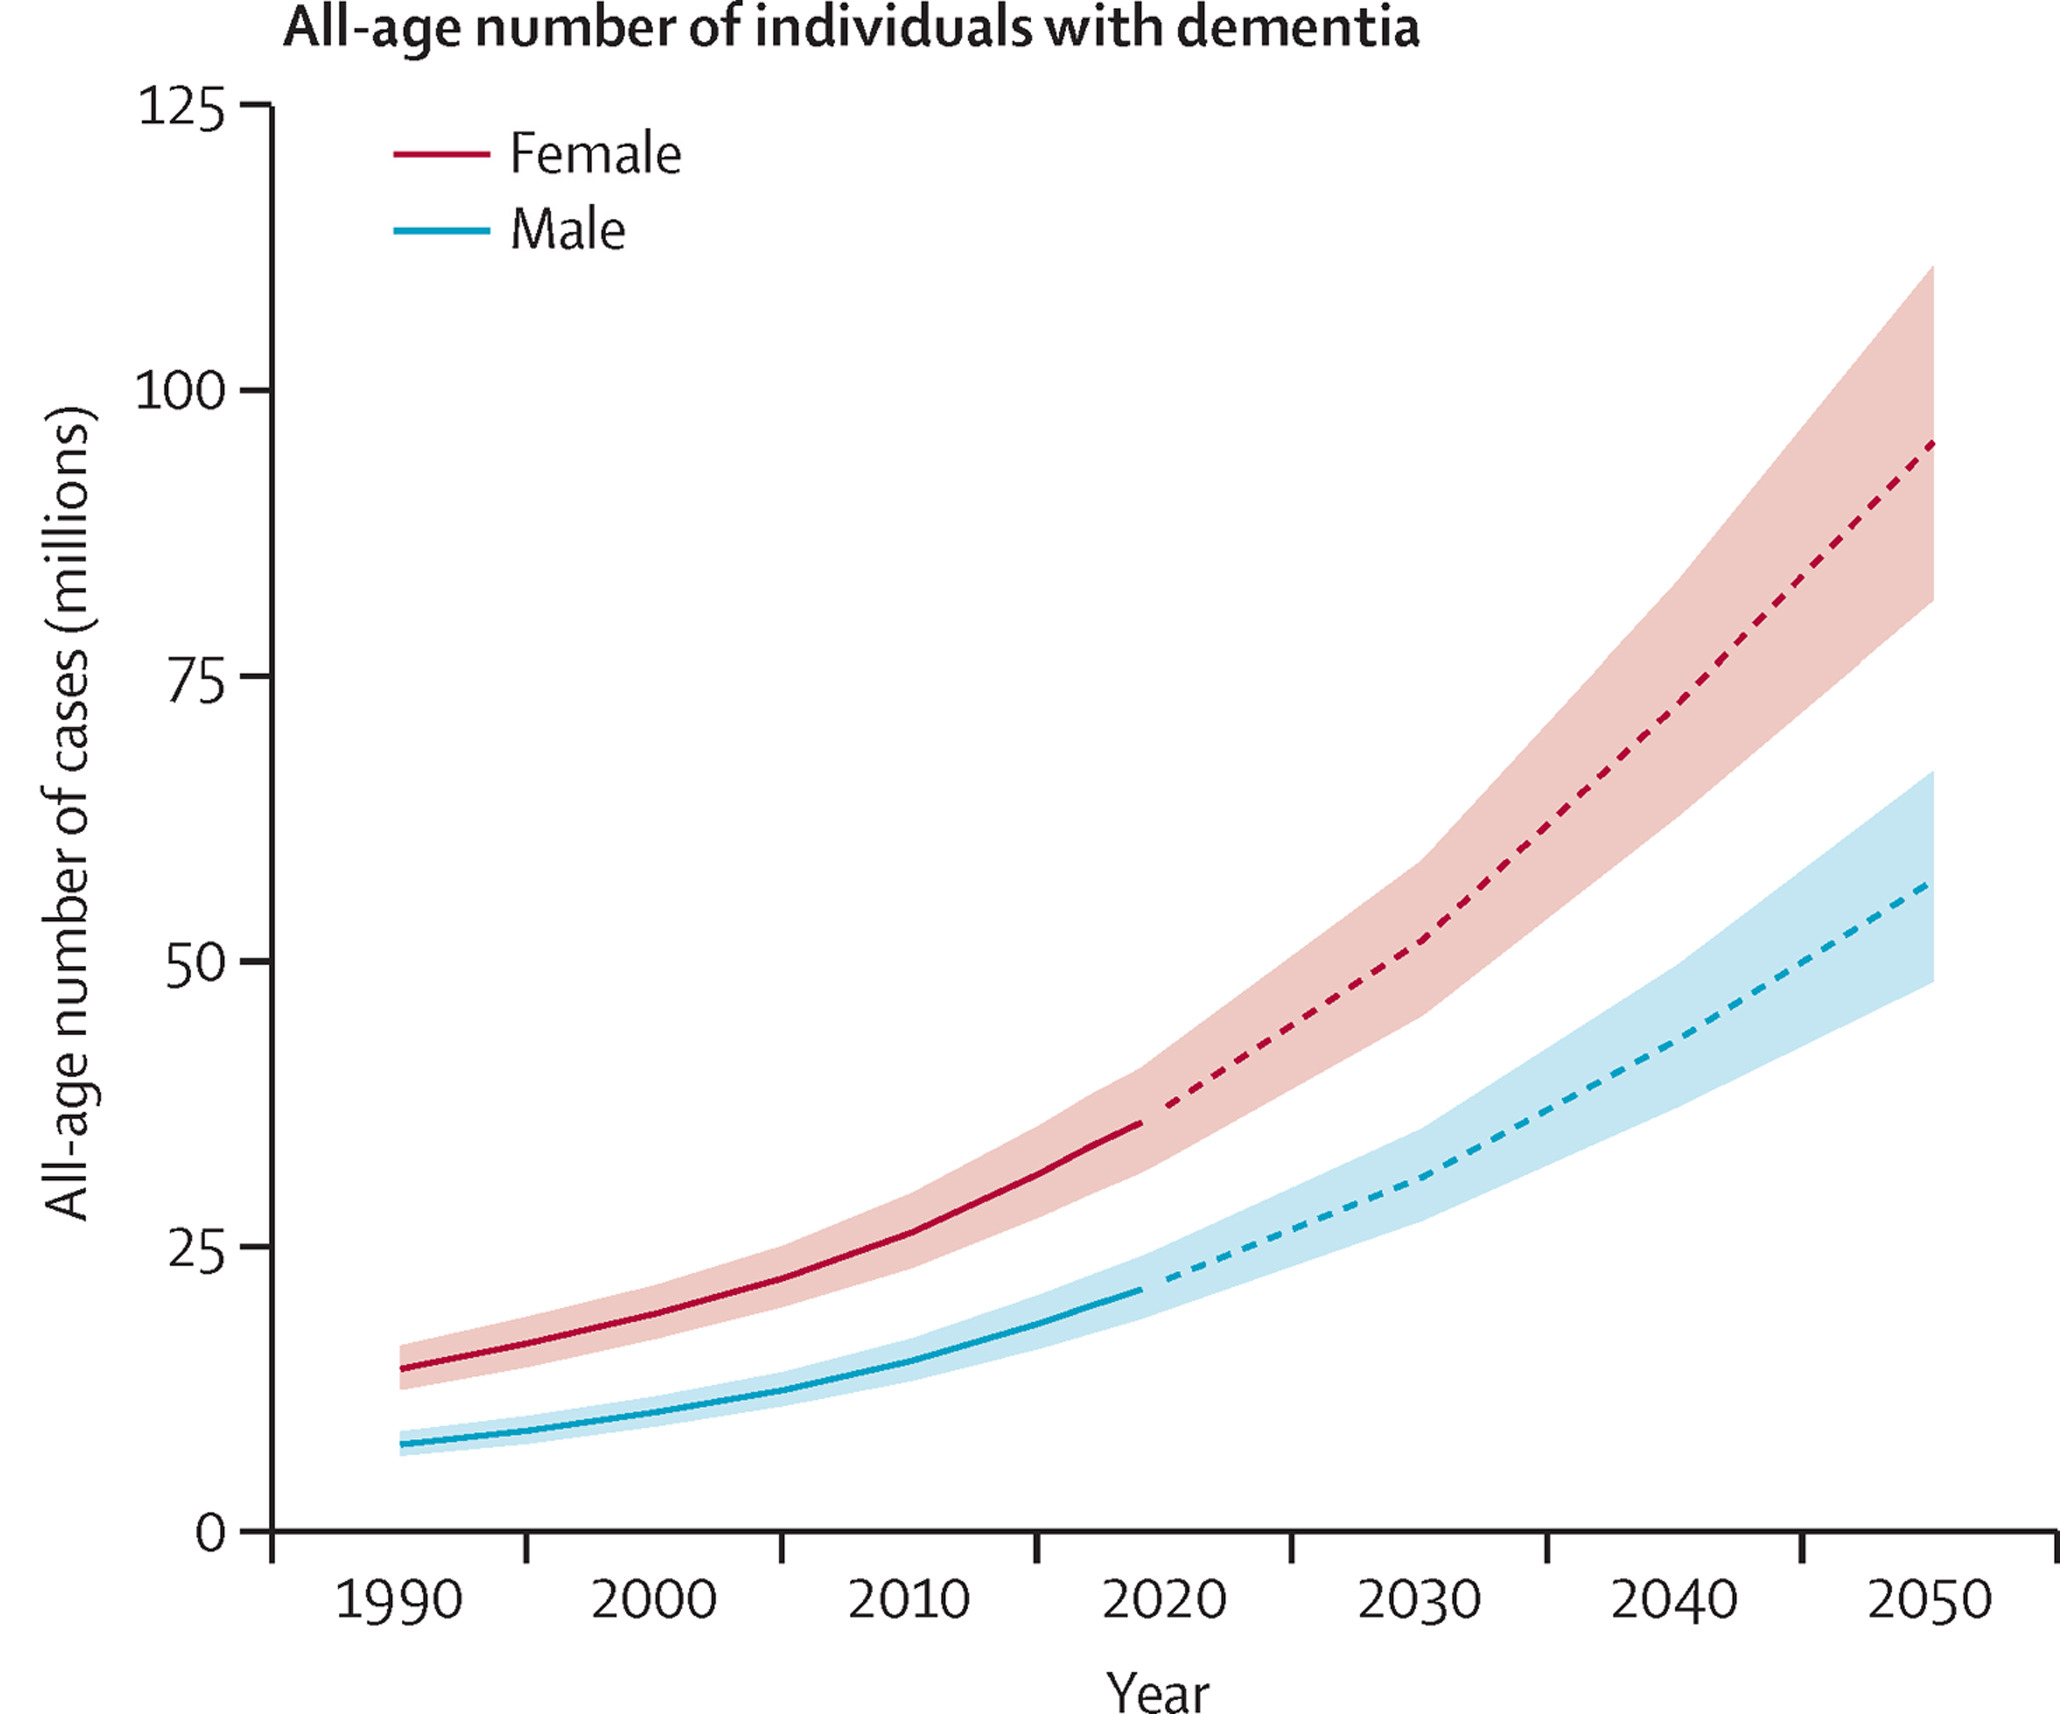
\includegraphics[width=6cm]{data/prevalence.jpg}
                };
                \node[anchor=south, font=\tiny, text width=10cm, align=flush center] at (0, -3.75) {
                    Global Burden of Disease Dementia Forecasting Collaborators (2022). Estimation of the global prevalence of dementia in 2019 and forecasted prevalence in 2050: an analysis for the Global Burden of Disease Study 2019. \textit{The Lancet Public Health}.
                };
            }
            \only<2>{
                \node[inner sep=0pt, draw=black] at (0, 0) {
                    
\includegraphics[width=6cm]{data/ema.png}
                };
            }
            \only<3>{
                \node[inner sep=0pt, draw=black] at (0, 0) {
                    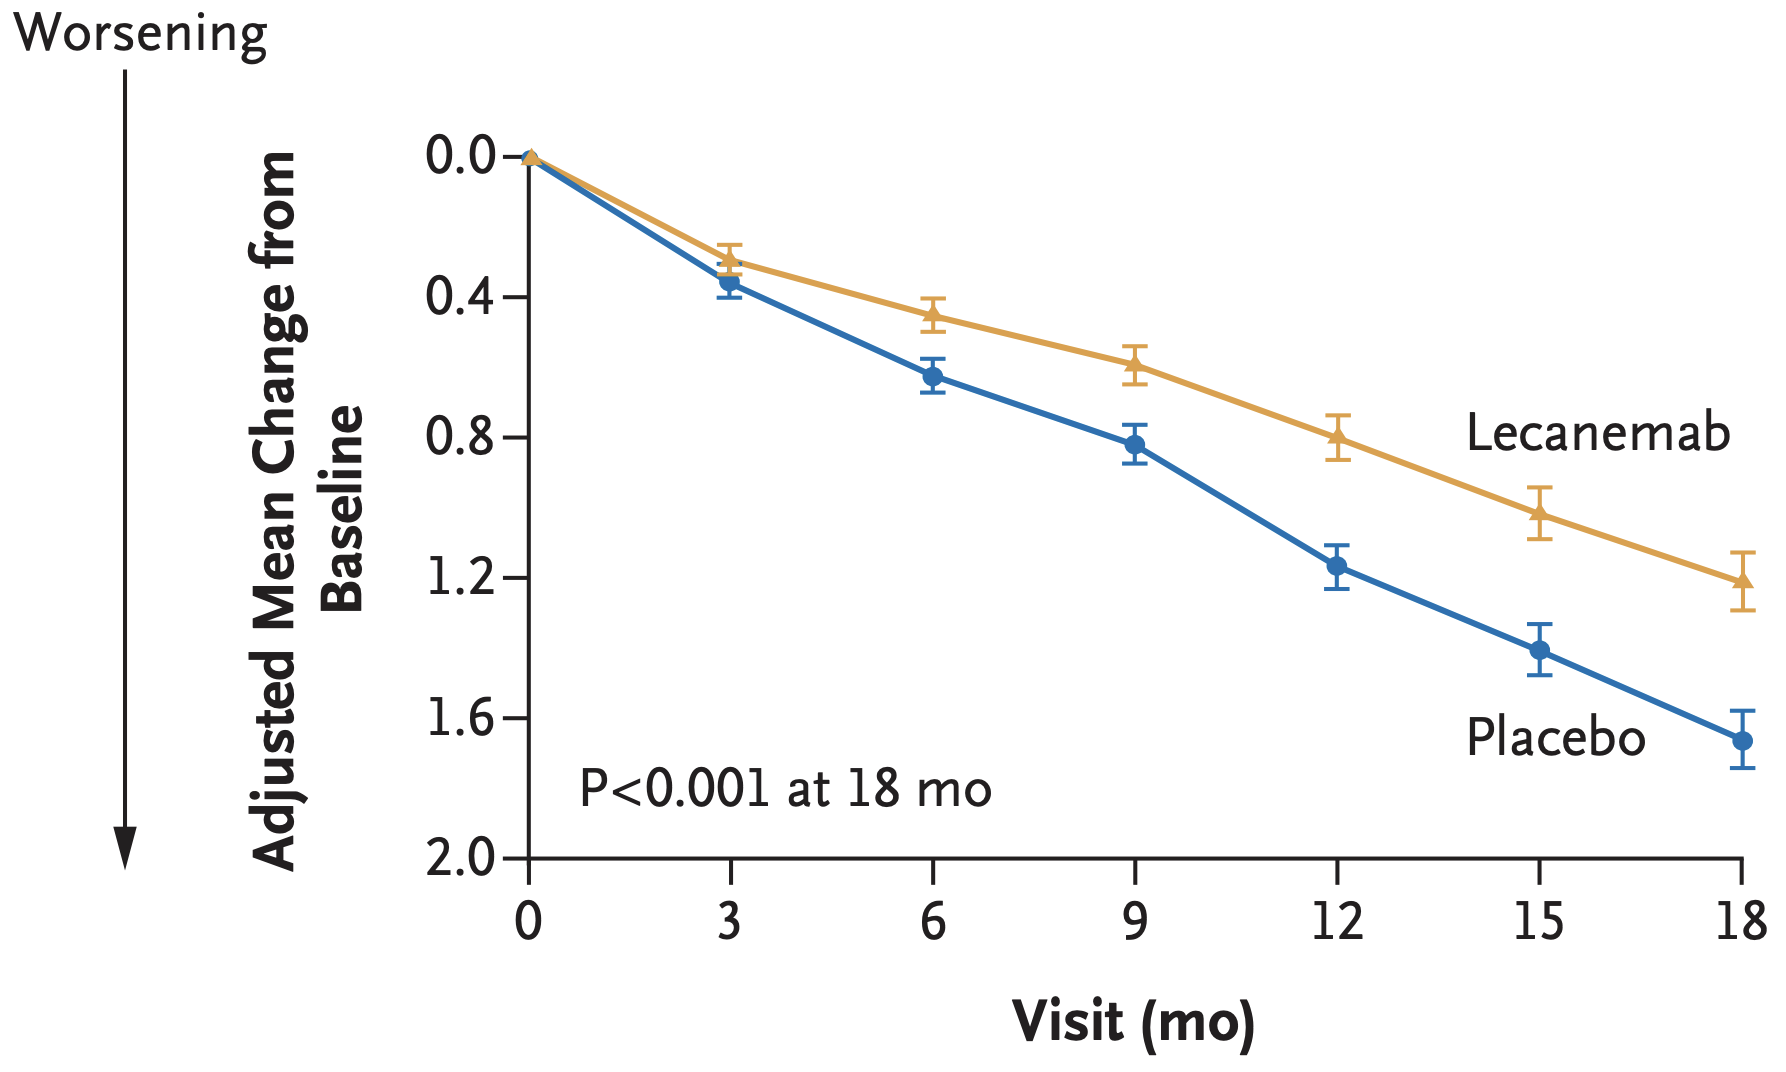
\includegraphics[width=8.5cm]{data/worsening.png}
                };
                \node[anchor=south, font=\tiny, text width=10cm, align=flush center] at (0, -3.75) {
                    Van Dyck, C. H., Swanson, C. J., Aisen, P., Bateman, R. J., Chen, C., Gee, M., ... \& Iwatsubo, T. (2023). Lecanemab in early Alzheimer’s disease. \textit{New England Journal of Medicine}.
                };
            }
            \only<4>{
                \node[] at (0, 0) {
                    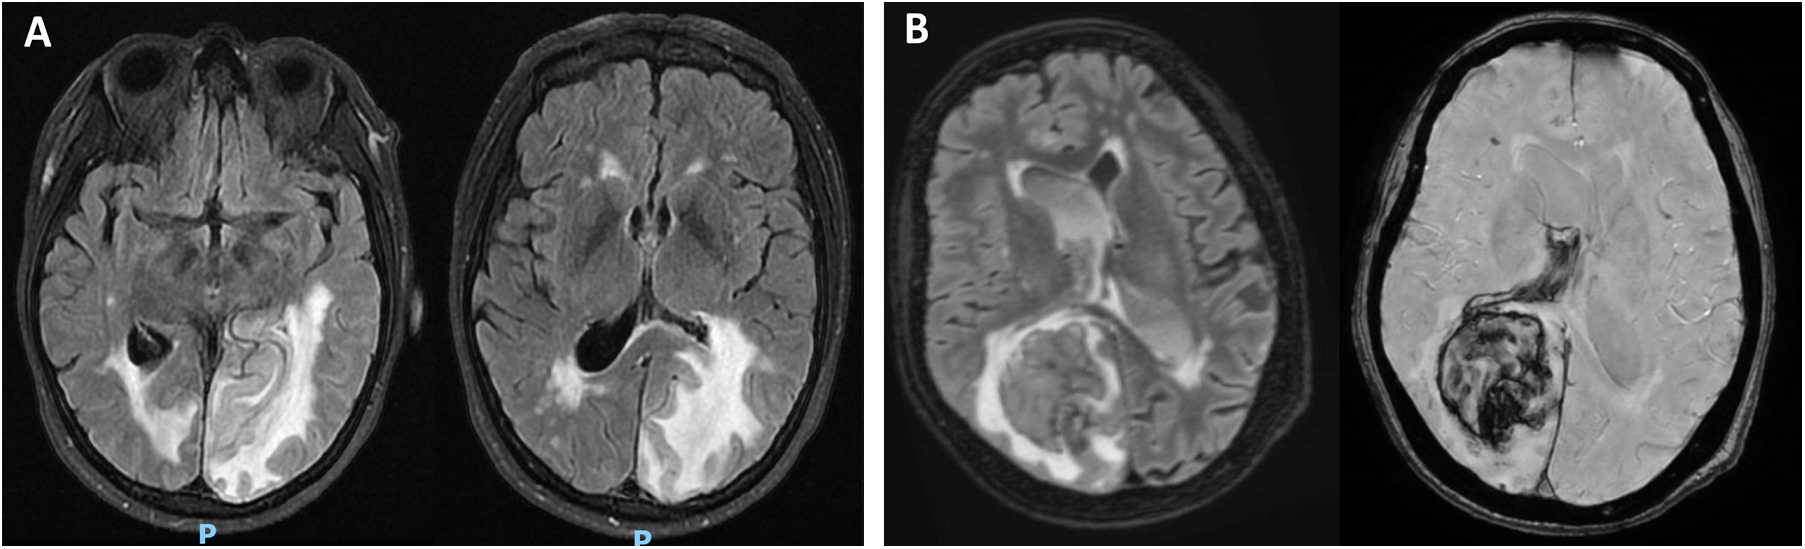
\includegraphics[width=10cm]{data/aria.jpg}
                };
                \node[anchor=south, font=\tiny, text width=10cm, align=flush center] at (0, -3.75) {
                    Villain, N., Planche, V., \& Levy, R. (2022). High-clearance anti-amyloid immunotherapies in Alzheimer's disease. Part 1: Meta-analysis and review of efficacy and safety data, and medico-economical aspects. \textit{Revue neurologique}.
                };
            }
        \end{tikzpicture}
    \end{frame}

    \begin{frame}{The baba.vision treatment support suite}
        \begin{tikzpicture}
            \node[] at (-5.25, 3.5) {};
            \node[] at (5.25, -3.5) {};

            \only<1-3>{
                \node[draw=black, inner sep=0pt, rounded corners=0.2cm] at (0, 0) {
                    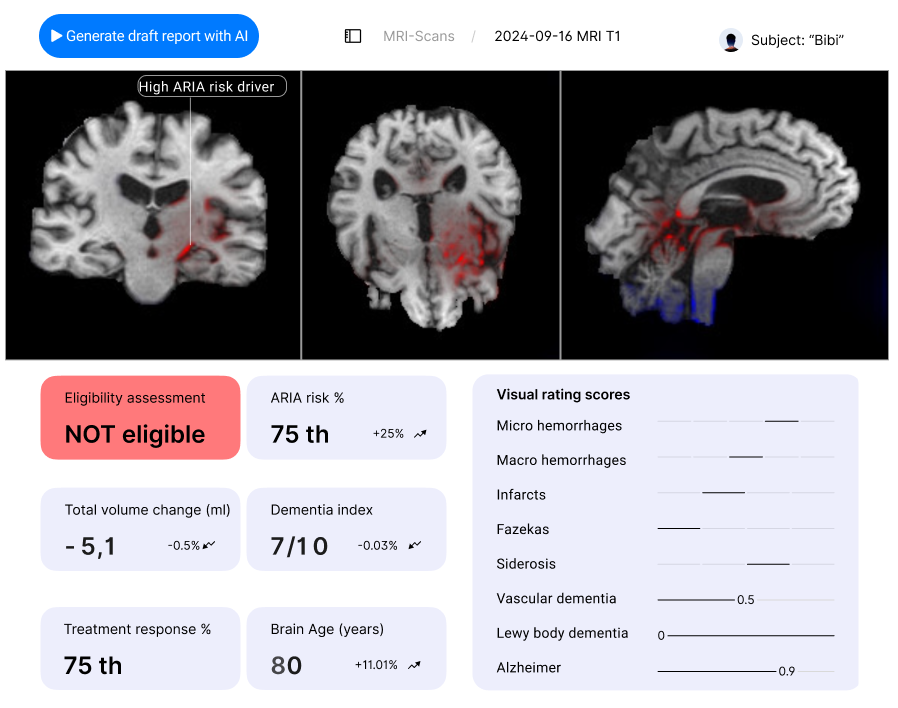
\includegraphics[width=8cm]{data/prototype.png}
                };
            }

            \only<2>{
                \node[minimum height=1.55cm, minimum width=3.4cm, draw=red, thick] at (1.93, -1.25) {};
                \node[minimum height=0.7cm, minimum width=1.8cm, draw=red, thick] at (-2.75, -1.56) {};
            }

            \only<3>{
                \node[minimum height=1cm, minimum width=3.4cm, draw=red, thick] at (1.93, -2.5) {};
                \node[minimum height=0.7cm, minimum width=1.8cm, draw=red, thick] at (-2.75, -0.57) {};
                \node[minimum height=0.7cm, minimum width=1.8cm, draw=red, thick] at (-0.92, -1.56) {};
                \node[minimum height=0.7cm, minimum width=1.8cm, draw=red, thick] at (-0.92, -2.62) {};
            }
        \end{tikzpicture}
    \end{frame}

    \begin{frame}{Explainable Artificial Intelligence}
        \begin{tikzpicture}
            \node[] at (-5.25, 3.5) {};
            \node[] at (5.25, -3.5) {};

            \only<1-2,4>{
                \cnn{-2.3}{1.5}{0.066}{0.15}{black}{1}
            }
            \only<2,4>{
                \inputside{-4}{1.5}{1.5cm}
                \node[
                    font=\linespread{0.9}\selectfont,
                    align=left,
                    anchor=west
                ] (output) at (3.4, 1.5) {
                    Dementia\\patient?
                };
                \cnnarrow{(input.east)}{($ (input.center) + (2, 0) $)}{black}
                \cnnarrow{($ (output.west) - (0.54, 0) $)}{($ (output.west) + (0.1, 0) $)}{black}
            }
            \visible<3>{
                \node[inner sep=2pt, fill=white, draw=black] at (0, 0) {
                    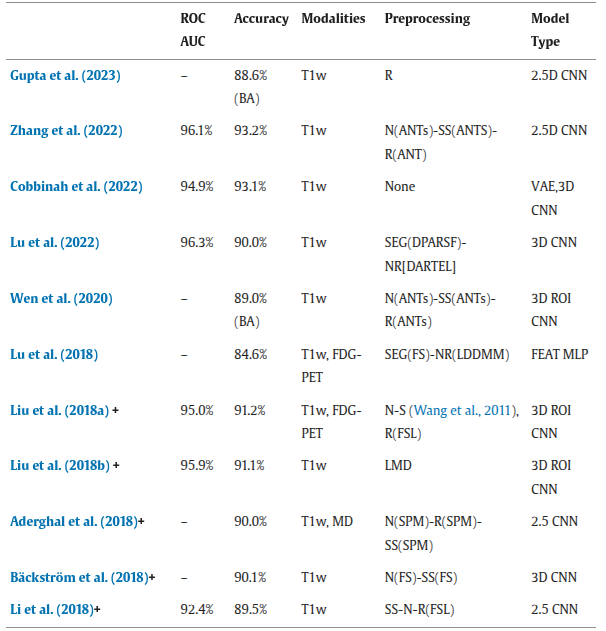
\includegraphics[width=5cm]{data/grodem.png}
                };
                \node[minimum width=0.6cm, minimum height=5.1cm, draw=red, thick] at (-0.35, 0) {};

                \node[anchor=south, font=\tiny, text width=10cm, align=flush center] at (0, -3.75) {
                    Grødem, et al., (2024). A minimalistic approach to classifying Alzheimer's disease using simple and extremely small convolutional neural networks. \textit{Journal of Neuroscience Methods}.
                };
            }
            \only<4>{
                \node[align=left, text width=7cm] at (0, -2) {
                    \begin{itemize}
                        \item[\textcolor{green}{+}] Produces very accurate predictions\\
                        \item[\textcolor{red}{-}] Very hard to understand
                    \end{itemize}
                };
            }
            \only<5>{
                \node[
                    font=\linespread{0.9}\selectfont,
                    align=left,
                    anchor=west
                ] (output) at (3.4, 1.5) {
                    Dementia\\patient?
                };
                \heatmapside{-4}{1.5}{1.5cm}
                \lrparrow{($ (input.center) + (2, 0) $)}{(input.east)}{black}
                \lrp{-2.3}{1.5}{0.066}{0.15}
                \lrparrow{($ (output.west) + (0.1, 0) $)}{($ (output.west) - (0.54, 0) $)}{black}
            }
            \only<6>{
                \node[label={[text depth=0]above:Explainable AI}] at (-2.25, 0) {
                    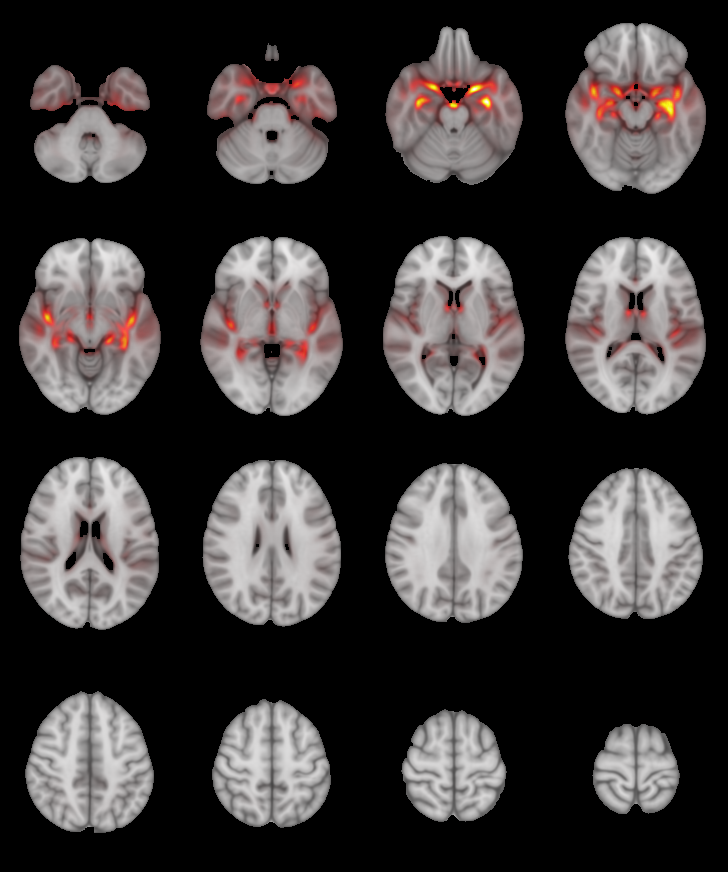
\includegraphics[width=0.31\textwidth]{data/dementia.png}
                };

                \node[label={[text depth=0]above:Human researchers}] at (2.25, 0) {
                    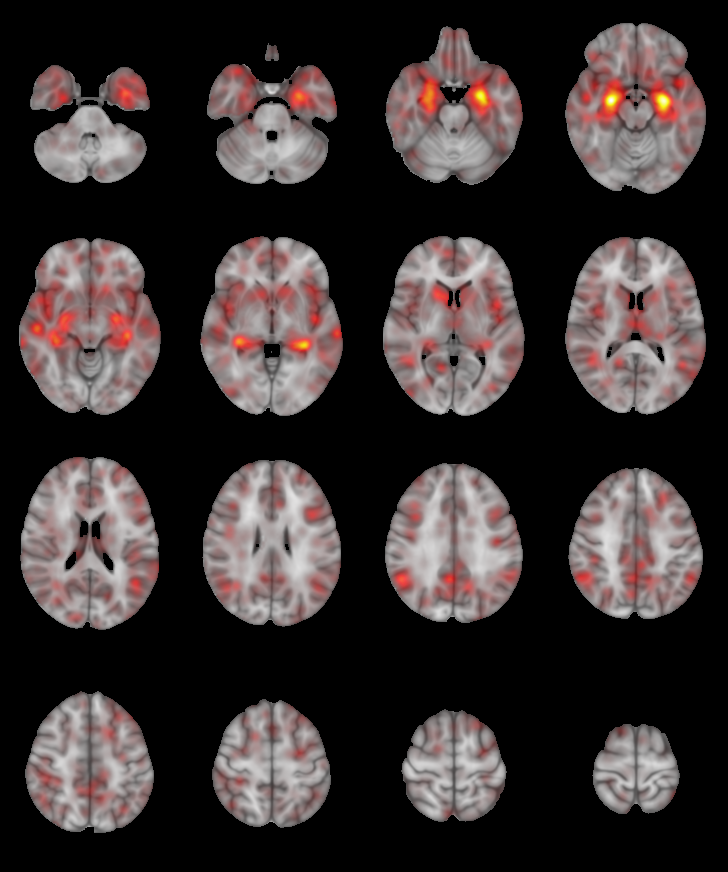
\includegraphics[width=0.31\textwidth]{data/ALE.png}
                };

                \node[anchor=south, font=\tiny, text width=10.5cm, align=flush center] at (0, -3.75) {
                    Leonardsen et al., (2024). Constructing personalized characterizations of structural brain aberrations in patients with dementia using explainable artificial intelligence, \textit{npj Digital Medicine}
                };
            }
        \end{tikzpicture}
    \end{frame}

    \begin{frame}{The baba.vision treatment support suite}
        \begin{tikzpicture}
            \node[] at (-5.25, 3.5) {};
            \node[] at (5.25, -3.5) {};

            \only<1-2>{
                \node[draw=black, inner sep=0pt, rounded corners=0.2cm] at (0, 0) {
                    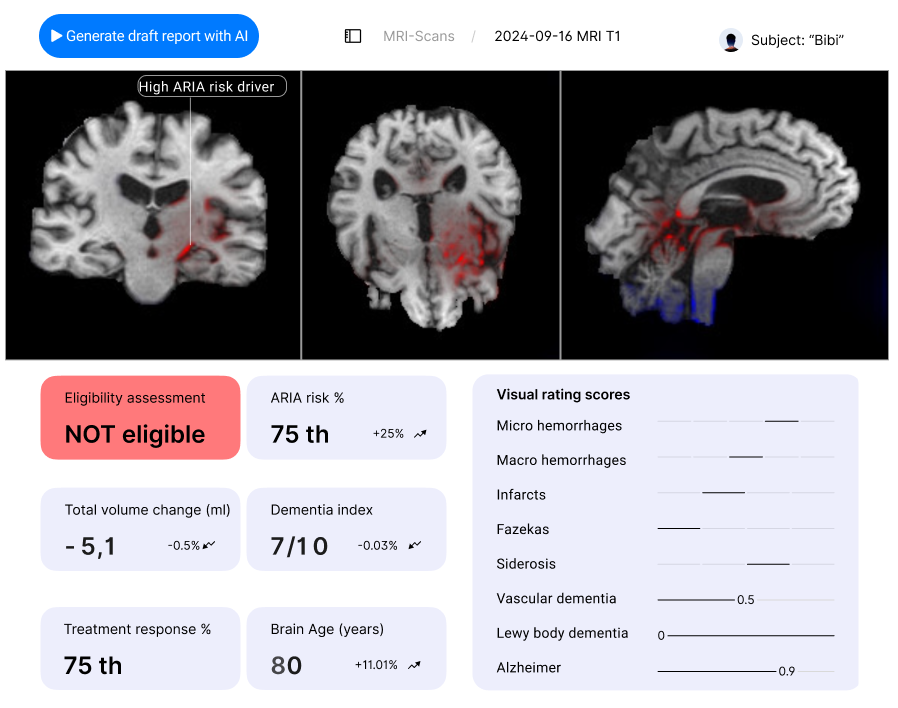
\includegraphics[width=8cm]{data/prototype.png}
                };
            }

            \only<1>{
                \node[minimum height=2.64cm, minimum width=7.95cm, draw=red, thick] at (-0.02, 1.24) {};
            }

            \only<2>{
                \node[minimum height=0.7cm, minimum width=1.8cm, draw=red, thick] at (-0.92, -0.57) {};
                \node[minimum height=0.7cm, minimum width=1.8cm, draw=red, thick] at (-2.75, -2.62) {};
            }
        \end{tikzpicture}
    \end{frame}

\end{document}
